\documentclass[12pt]{article}
\usepackage{fullpage,enumitem,amsmath,amssymb,graphicx,dsfont,setspace, multicol, pdfpages, graphicx, caption}

\begin{document}

\begin{center}

{\Large \textbf{Reconstructing 3D Structure from Amazon Product Images}}

\begin{multicols}{3}
Jason van der Merwe\\
jasonvdm@stanford.edu\\
\columnbreak
Andrew Giel\\
agiel@stanford.edu\\
\columnbreak
Bridge Eimon\\
beimon@stanford.edu\\
\end{multicols}
CS 231A Stanford University\\
December 8, 2013\\
\end{center}
\noindent\rule{16.5cm}{0.4pt}\\
{\large \textbf{Abstract}}\\
This paper presents the methods we explored for three dimensional stuctural reconstruction from two dimensional product images on Amazon.com. We began with our own images of a volleyball for a proof of concept. Using SURF and RANSAC, we found correspondence points among the images. After we retrieved these points, we computed structure from motion (SfM) among image pairs. To stitch the SfMs from image pairs together, we used RANSAC and the SURF descriptors for the points in the 3D point cloud to combine the point clouds from each image pair together. After this step, we were able to plot the 3D structure. Our method produced accurate results for the volleyball images, however, we were unable to successfully plot the structures for Amazon products for a variety of reasons. One obstacle is that Amazon product images are taken with a large amount of rotation between each image, so the amount of redundancy is low. Additionally, most products exhibit considerable symmetry, so the performance struggles from SURF and RANSAC. Our paper further analyzes the issus we encountered and the steps that Amazon could take in order to ensure their product images could be used for 3D reconstruction.\\
\begin{multicols}{2}
{\noindent \large \textbf{1. Introduction}}\\
This project, reconstructing 3D models from Amazon product images, is the first step of a larger goal to build a database of 3D objects by crawling the web.  This database can then be used to assist in many other object detection tasks, such as identifying objects in your home or from a cell phone camera.  One important component of making such a system is to build 3D object models from multiple views of web images. SFM is generally performed using a number of images carefully taken of the same object.  Can we use SfM from product images taken by different users?  Amazon often has a collection of images for each object uploaded by different users.  These views were all taken with different cameras in different lighting / backgrounds, which adds a challenge.  Can we combine these images to create 3D object models?
\\\\
{\large \textbf{2.1 Previous Work}}\\
Recreating the structure of an object from a set of images has been explored by many instances of previous research, even in a completely unsupervised and automatic fashion. \\
\indent In fact, the concept of taking images available online of the same object or scene and then reconstructing the three dimensional properties from these images has been achieved by previous research. In a paper entitled `Photo Tourism: Exploring Photo Collections in 3D', Noah Snavely presents a system that retrieves images of famous landmarks and then infers the structure of the landmarks in three dimensions as well as the pose and location of the cameras which captured the images. After establishing correspondences, Navely utlized the Levenberg-Marquardt algorithm to solve the least-squares problem of sparse bundle adjustment. Once this structure known, Snavely and his team were able to rerender the scene as well as the position of the cameras. \\
\indent A key portion of the reconstruction process, as mentioned above, is establishing correspondences between the images. This can be achieved via expensive manual annotation or by solving the longstanding correspondence problem. David Lowe's work on the Scale-Invariant Feature Transform (SIFT) helped to address this cardinal problem in the vision commmunity. By implementing a difference-of-Gaussian function to identify points of interest in the images, Lowe was able to then localize and establish their dominant orientation. Once the keypoints were defined and desciptors established, Lowe utilized best-bin-first search in order to find the best match from any one keypoint of an image to a keypoint from another image, using Euclidean distance as the ranking metric. In order to determine the probability of a match, Lowe used the ratio of the distance to the best match to the distance of the second best match, eliminating matches with a distance ratio over a certain threshold. Combining this methodology with a model-generating procedure such as Random Sample Consensus (RANSAC) has proven to be effective in estimating the correspondence problem, and was utilized in our implementation as well. \\
\indent Given a set of correspondences, recovering the structure from motion is a non-trivial problem. Tomasi and Kanade, in their seminal paper, present a method for extracting scene geometry and camera motion from a matrix $W$ derived from the measurements and correspondences. Tomasi and Kanade realized that the points are represented within a low-dimension subspace of $W$, allowing them to be extracted via Singular Value Decomposition. This method performs best when used on points without occlusions, yet methods are presented to extrapolate measurements. \\
\indent In 2005, Lowe published a paper titled `Unsupervised 3D Object Recognition and Reconstruction in Unordered Datasets' in which he outlined a procedure to recreate the 3D structure of objects using his SIFT feature descriptors, RANSAC, and spare bundle adjustment without any user input. He proved that such a process was possible, giving a technical foundation for our experiments with Amazon.\\\\
{\large \textbf{2.2 Advancements}}\\
Our experiments take the concepts presented by the Snavely Photo Tourism paper and Lowe's unsupervised reconstruction paper and test the limits to which these concepts can be applied, by attempting to reconstruct products on Amazon. Product photos on Amazon present a number of challenges which make the reconstruction process difficult, which is elaborated in the Error Analysis section. Testing methods presented in these papers on imperfect, noisy, and occluded data helps to define the limits of our ability to successfully recreate three dimensional structure. Additionally, by attempting to apply this sort of technique to a new domain and create a new product for Amazon we can make a commercial impact and not just an academic or theoretical assessment. \\\\
{\large \textbf{3.1 Technical Summary}}\\
We implemented our system incrementally, starting first by testing our reconstruction on manually annotated correspondences with images we took ourselves in a controlled environment. Our SfM is computed using the Tomasi-Kanade factorization algorithm. This allowed us to have a full measurement matrix for our Tomasi-Kanade. Once this was verified to work on with manually annotated images of our own we implemented automatic correspondence using SIFT, SURF, and ORB descriptors, matching using Euclidean distance and verifying by comparison to the second closest match. In order to refine our correspondence matches we used RANSAC, experimenting with different thresholds. In the case where we have multiple point clouds (SfMs) corresponding to structures inferred from a pair of two images, we combined these point clouds using a similar procedure. Given a set of points in three dimensions and their corresponding desciptors (SIFT, SURF, ORB), we determined the best match between these clouds via RANSAC. Using RANSAC on the three dimensional points, we generate a three dimensonal homography. This homography can be used to translate the points in one point cloud to the points in another point cloud, merging the structures captured. Once we tuned our system to work on our own images, we tested on Amazon images. \\
\indent Our method can be broken down into 4 discrete steps: description, detection, inference of structure, and merging of structures. \\\\
{\large \textbf{3.2 Description}}\\
In order to obtain keypoints and descriptors from images, we tried SIFT, SURF and ORB. After experimenting, we found that SURF obtained the most keypoints and descriptors for our images. We utilized the OpenCV implementations of these algorithms. These functions returned a 128-dimension descriptor vector for every keypoint in the image plane. These keypoints and descriptors were then passed to our matching algorithms.\\\\
{\large \textbf{3.3 Detection}}\\
{\large \textbf{3.4 Structure}}\\
Once we have obtained a set of geometrically consistent matches, we want to obtain the structure in a point cloud via the Tomasi-Kanade algorithm. \\
\indent The first step in this process is to center the image points. This is achieved by subtracting the centroid of the points from each of the points. More formally, for every point $x_{ij}$ on camera $i$ we subtract $\bar{x_{i}}$. 
\[\hat{x}_{ij} = x_{ij} - \bar{x}_{i}\]
\[\hat{x}_{ij} = x_{ij} - {{1}\over{n}} \sum_{k=1}^{n} x_{ik}\]
Where $n$ is the number of points on one image. Note that this can be expressed equivelently as a function of the camera in the affine model. 
\[x_{ij} = A_{i}X_{k} + b_{i}\]
\[\hat{x}_{ij} = A_{i}X_{j} + b_{i} - {{1}\over{n}} \sum_{k=1}^{n} (A_{i}X_{k} + b_{i})\]
\[\hat{x}_{ij} = A_{i}(X_{j}  - {{1}\over{n}} \sum_{k=1}^{n} X_{k})\]
This means that every point $\hat{x}_{ij} = A_{i}\hat{X}_{j}$, which means that if we put the center of the world coordinate system as the centroid, $\hat{x}_{ij} = A_{i}\hat{X}_{j} = A_{i}X_{j}$, allowing for factorization to occur. \\
\indent With our newly centered data we can perform the factorization that is the key insight of the Tomasi-Kanade algorithm. First, it is necessary to create a measurement matrix $D$ of size (2$m \times n$), where $m$ is the number of frames and $n$ is again the number of points. The reason the factor of two is present is that the first $m$ dimensions of the matrix are the x coordinates of the points in the image plane, while the remaining $m$ dimensions are the y coordinates. \\
\indent	With our measurement matrix $D$, we know both the structure and motion are obtainable via factorization. The measurements $D$ can be broken into $MS$, where $M$ is the motion (camera matrices and orientations) of size (2$m \times$3) and $S$ is the structure matrix (3 dimensional points $X_{j}$) of size (3$\times n$). We cannot determine $MS$ by a simple fatorization, but we can perform Singular Value Decomposition (SVD) to have access to the component matrices, $D = UWV^T$. We can recover $MS$ by taking portions of the SVD components. $M$ = $U_{3}$, or the first 3 columns of $U$. Similarly, $S$ = $W_{3}V^{T}_{3}$ or the first 3 columns of the the first three rows of $W$ and the first 3 dimensions of $V^{T}$. The resulting $S$, of size (3$\times n$), is a column matrix of the points, our intended result. 
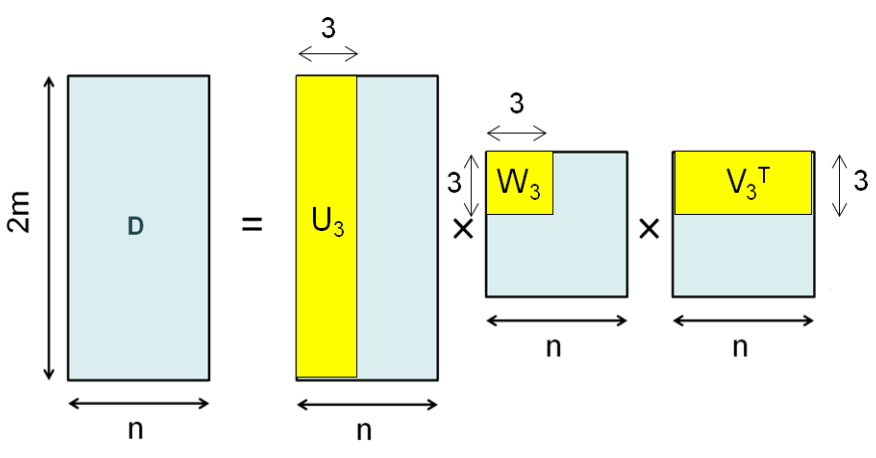
\includegraphics[width=0.5\textwidth]{images/SVD_of_D.png}
\\\\
{\large \textbf{3.5 Merging Structures}}\\
Once we computed our multiple point clouds using SfM, the last step was to aggregate all the points into one output space. In order to do this, we used a modified version of RANSAC applied to the points in 3D space in our point clouds. To merge two point clouds together, we used the SURF descriptors of the image common to both point clouds to find the matches between points in the point clouds. The next step is to use RANSAC to find a 4x4 homography which maps points from the first point cloud to the second with the largest number of inliers. $H$ is a homogenized 4x4 matrix, so we homogenized the first point cloud, the calculated the points from the first cloud into the output space of the second point cloud by $P_2$ = $H\times homogenizedP_1$. Once we then dehomogenized these points, we added them into the output space of the second point cloud, resulting in an image containing an aggregation of both point clouds. We then take two of these combined set of point clouds and combine them as well until we have a single point cloud containing all our keypoints.\\\\
{\large \textbf{4. Experiments}}\\
We tested our implementation on many different sets of images. This includes images we took ourself, images taken from Amazon, different objects, different resolutions, and image sets with different degrees of rotation between individual images. 


\end{multicols}
\end{document}